%!TEX root = ../booklet.tex
% ^ leave for LaTeXTools build functionality

\begin{puzzle}
Vera and Horace are playing a game called \textbf{Domineering}. The game is
played on a rectangular grid like a chessboard, though it usually isn't quite as
big. In the game, players take turns laying down dominoes, without overlapping
any previously laid dominos. Vera goes first,
and she may only lay her dominoes vertically. Horace goes second, and he may
only lay a domino horizontally. The players take turns until one player loses
because he or she cannot make a legal move. The other player is then the winner.

In the following scenarios, write down the specified numbers going across
first, then down. Then use these numbers to shift the appropriate letters.
\begin{center}
  \fbox{\begin{minipage}{.7\linewidth}
    \textbf{Example} Vera has won the following game because it is Horace's
    turn and he cannot lay a horizontal domino.
    \begin{center}
    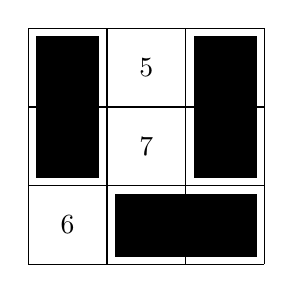
\begin{tikzpicture}
    \draw (0,0) grid (3,3);
    \node at (1.5,2.5) {5};
    \node at (1.5,1.5) {7};
    \node at (.5,.5) {6};
    \fill (0.1,1.1) rectangle (0.9,2.9);
    \fill (2.1,1.1) rectangle (2.9,2.9);
    \fill (1.1,0.1) rectangle (2.9,0.9);
    \end{tikzpicture}
    \end{center}
    If we use the numbers not covered by a domino, we get the following:
    \begin{center}
    \letterBoxFilled{T+5=}{Y}
    \letterBoxFilled{X+7=}{E}
    \letterBoxFilled{M+6=}{S}
    \end{center}
  \end{minipage}}
\end{center}

\vfill

\begin{enumerate}
  \item
    No dominos have been played on the below board.
    Suppose Horace wins after making two moves.
    \textbf{Use the only number not covered by a domino.}
    \begin{center}
    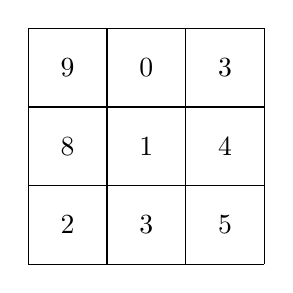
\begin{tikzpicture}
    \draw (0,0) grid (3,3);
    \node at (.5,2.5) {9};
    \node at (.5,1.5) {8};
    \node at (.5,.5) {2};
    \node at (1.5,2.5) {0};
    \node at (1.5,1.5) {1};
    \node at (1.5,.5) {3};
    \node at (2.5,2.5) {3};
    \node at (2.5,1.5) {4};
    \node at (2.5,.5) {5};
    \end{tikzpicture}
    \end{center}
    \begin{center}
    \letterBox{Z+?=}
    \end{center}

\vfill
\newpage
  \item
    No dominos have been played on the below board.
    Suppose Vera makes her first move within the left column,
    and Horace wins after making his first move.
    \textbf{Use the two numbers Horace covered with his only domino.}
    \begin{center}
    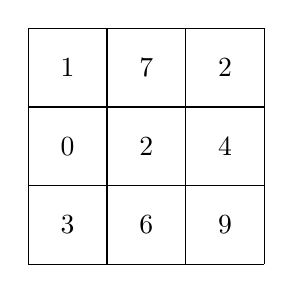
\begin{tikzpicture}
    \draw (0,0) grid (3,3);
    \node at (.5,.5) {3};
    \node at (1.5,.5) {6};
    \node at (2.5,.5) {9};
    \node at (.5,1.5) {0};
    \node at (.5,2.5) {1};
    \node at (1.5,1.5) {2};
    \node at (1.5,2.5) {7};
    \node at (2.5,1.5) {4};
    \node at (2.5,2.5) {2};
    \end{tikzpicture}
    \end{center}
    \begin{center}
    \letterBox{J+?=}
    \letterBox{W+?=}
    \end{center}

\vfill

  \item
    Vera and Horace have already played one domino each on the below board.
    Suppose Vera is able to play three additional dominos, but ends up losing.
    \textbf{Use the six numbers Vera covered with her
    three additional dominos.}
    \begin{center}
    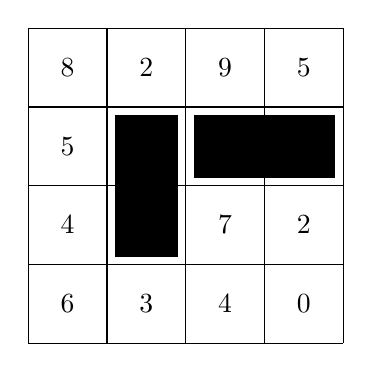
\begin{tikzpicture}
    \draw (0,0) grid (4,4);
    \node at (.5,.5) {6};
    \node at (.5,1.5) {4};
    \node at (.5,2.5) {5};
    \node at (.5,3.5) {8};
    \node at (1.5,.5) {3};
    \node at (1.5,3.5) {2};
    \node at (2.5,.5) {4};
    \node at (2.5,1.5) {7};
    \node at (2.5,3.5) {9};
    \node at (3.5,.5) {0};
    \node at (3.5,1.5) {2};
    \node at (3.5,3.5) {5};
    \fill (1.1,1.1) rectangle (1.9,2.9);
    \fill (2.1,2.1) rectangle (3.9,2.9);
    \end{tikzpicture}
    \end{center}
    \begin{center}
    \letterBox{W+?=}
    \letterBox{W+?=}
    \letterBox{F+?=}
    \letterBox{Y+?=}
    \letterBox{I+?=}
    \letterBox{O+?=}
    \end{center}

\vfill

  \item
    Vera and Horace have already played one domino each on the below board.
    Suppose Horace wins after both players play one additional domino.
    \textbf{Use the four numbers Vera and Horace covered with those
    two additional dominos.}
    \begin{center}
    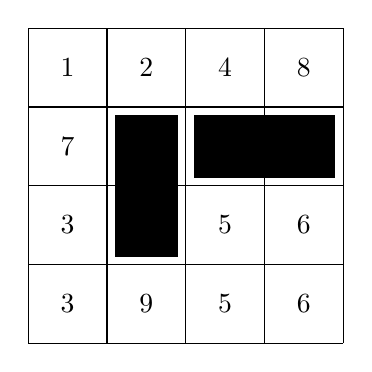
\begin{tikzpicture}
    \draw (0,0) grid (4,4);
    \node at (.5,.5) {3};
    \node at (.5,1.5) {3};
    \node at (.5,2.5) {7};
    \node at (.5,3.5) {1};
    \node at (1.5,.5) {9};
    \node at (1.5,3.5) {2};
    \node at (2.5,.5) {5};
    \node at (2.5,1.5) {5};
    \node at (2.5,3.5) {4};
    \node at (3.5,.5) {6};
    \node at (3.5,1.5) {6};
    \node at (3.5,3.5) {8};
    \fill (1.1,1.1) rectangle (1.9,2.9);
    \fill (2.1,2.1) rectangle (3.9,2.9);
    \end{tikzpicture}
    \end{center}
    \begin{center}
    \letterBox{O+?=}
    \letterBox{B+?=}
    \letterBox{Y+?=}
    \letterBox{Y+?=}
    \end{center}

\vfill
\newpage

  \item
    Vera and Horace have already played two dominoes each on the below board.
    \textbf{Use the only number which must be covered by either Horace or
    Vera during any completion of this game.}
    \begin{center}
    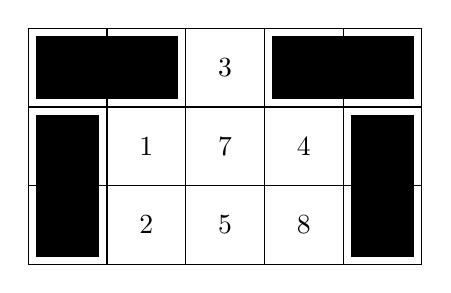
\begin{tikzpicture}
    \draw (0,0) grid (5,3);
    \node at (.5,2.5) {9};
    \node at (.5,1.5) {8};
    \node at (.5,.5) {2};
    \node at (1.5,2.5) {0};
    \node at (1.5,1.5) {1};
    \node at (1.5,.5) {2};
    \node at (2.5,2.5) {3};
    \node at (2.5,1.5) {7};
    \node at (2.5,.5) {5};
    \node at (3.5,2.5) {3};
    \node at (3.5,1.5) {4};
    \node at (3.5,.5) {8};
    \node at (4.5,2.5) {3};
    \node at (4.5,1.5) {4};
    \node at (4.5,.5) {5};
    \fill (0.1,2.1) rectangle (1.9,2.9);
    \fill (0.1,0.1) rectangle (0.9,1.9);
    \fill (4.1,0.1) rectangle (4.9,1.9);
    \fill (3.1,2.1) rectangle (4.9,2.9);
    \end{tikzpicture}
    \end{center}
    \begin{center}
    \letterBox{T+?=}
    \end{center}

  \item
    Vera and Horace have already played two dominoes each on the below board.
    Horace can now force Vera to lose unless she makes one specific move.
    \textbf{Use the two numbers Vera should cover with her next move.}
    \begin{center}
    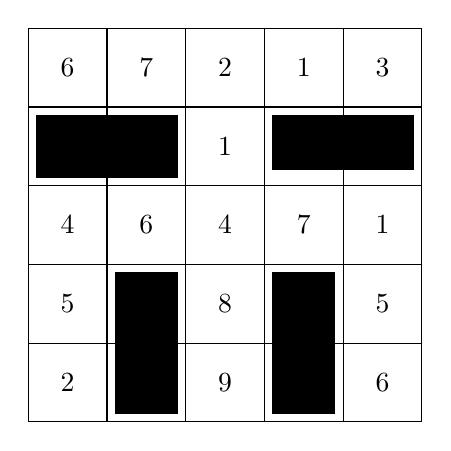
\begin{tikzpicture}
    \draw (0,0) grid (5,5);
    \node at (.5,.5) {2};
    \node at (.5,1.5) {5};
    \node at (.5,2.5) {4};
    \node at (.5,4.5) {6};
    \node at (1.5,2.5) {6};
    \node at (1.5,4.5) {7};
    \node at (2.5,.5) {9};
    \node at (2.5,1.5) {8};
    \node at (2.5,2.5) {4};
    \node at (2.5,3.5) {1};
    \node at (2.5,4.5) {2};
    \node at (3.5,2.5) {7};
    \node at (3.5,4.5) {1};
    \node at (4.5,.5) {6};
    \node at (4.5,1.5) {5};
    \node at (4.5,2.5) {1};
    \node at (4.5,4.5) {3};
    \fill (0.1,3.1) rectangle (1.9,3.9);
    \fill (3.1,3.2) rectangle (4.9,3.9);
    \fill (1.1,0.1) rectangle (1.9,1.9);
    \fill (3.1,0.1) rectangle (3.9,1.9);
    \end{tikzpicture}
    \end{center}
    \begin{center}
    \letterBox{R+?=}
    \letterBox{P+?=}
    \end{center}
\end{enumerate}

\vfill

Combine these shifted letters together to form a message.
\textbf{Report the decoded message to Game HQ for \(100\) Victory Points!}

\vfill

\begin{center}
    \letterBox{}
    \letterBox{}
    \letterBox{}
    \letterBox{}
    \letterBox{}
    \letterBox{}
    \letterBox{}
\end{center}
\begin{center}
    \letterBox{}
    \letterBox{}
    \letterBox{}
    \letterBox{}
    \letterBox{}
    \hspace{1em}
    \letterBox{}
    \letterBox{}
    \letterBox{}
    \letterBox{}
\end{center}

\vfill
\end{puzzle}

\begin{extraPuzzle}
  Vera and Horace decide to play Domineering on a $6 \times 6$ board.
  There are 36 squares on the board, so at most 18 dominoes can be played.
  Vera and Horace wonder what is the smallest number of dominoes that can be
  played in a completed game. For example, no matter what dominos Vera and
  Horace play during their first turns, Vera still has another legal
  move available. But it's possible to play a complete
  game where Horace makes the last move, and Vera cannot play any vertical
  dominoes, even though there is some uncovered space for a horizontal
  domino.

    \begin{center}
    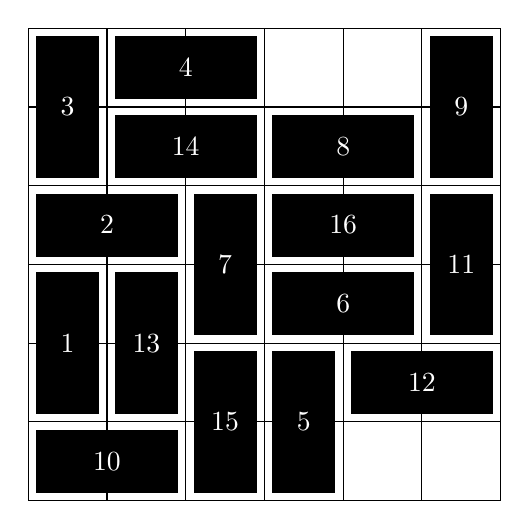
\begin{tikzpicture}
    \draw (0,0) grid (6,6);
    \fill (0.1,1.1) rectangle (0.9,2.9);
    \node[text=white] at (0.5,2) {1};
    \fill (0.1,3.1) rectangle (1.9,3.9);
    \node[text=white] at (1,3.5) {2};
    \fill (0.1,4.1) rectangle (0.9,5.9);
    \node[text=white] at (0.5,5) {3};
    \fill (1.1,5.1) rectangle (2.9,5.9);
    \node[text=white] at (2,5.5) {4};
    \fill (3.1,0.1) rectangle (3.9,1.9);
    \node[text=white] at (3.5,1) {5};
    \fill (3.1,2.1) rectangle (4.9,2.9);
    \node[text=white] at (4,2.5) {6};
    \fill (2.1,2.1) rectangle (2.9,3.9);
    \node[text=white] at (2.5,3) {7};
    \fill (3.1,4.1) rectangle (4.9,4.9);
    \node[text=white] at (4,4.5) {8};
    \fill (5.1,4.1) rectangle (5.9,5.9);
    \node[text=white] at (5.5,5) {9};
    \fill (0.1,0.1) rectangle (1.9,0.9);
    \node[text=white] at (1,0.5) {10};
    \fill (5.1,2.1) rectangle (5.9,3.9);
    \node[text=white] at (5.5,3) {11};
    \fill (4.1,1.1) rectangle (5.9,1.9);
    \node[text=white] at (5,1.5) {12};
    \fill (1.1,1.1) rectangle (1.9,2.9);
    \node[text=white] at (1.5,2) {13};
    \fill (1.1,4.1) rectangle (2.9,4.9);
    \node[text=white] at (2,4.5) {14};
    \fill (2.1,0.1) rectangle (2.9,1.9);
    \node[text=white] at (2.5,1) {15};
    \fill (3.1,3.1) rectangle (4.9,3.9);
    \node[text=white] at (4,3.5) {16};
    \end{tikzpicture}
    \end{center}

  Sketch another completed board
  below with horizontal and vertical dominos,
  \textit{numbering the order in which they are played}. Submit your
  completed board to Game HQ before the end of the game.
  Boards which are illegally constructed or
  incomplete will be disqualified.
  \textbf{The team(s) submitting a valid board using the
  \textit{least} number of dominoes will earn \(50\) Victory Points.}

    \begin{center}
    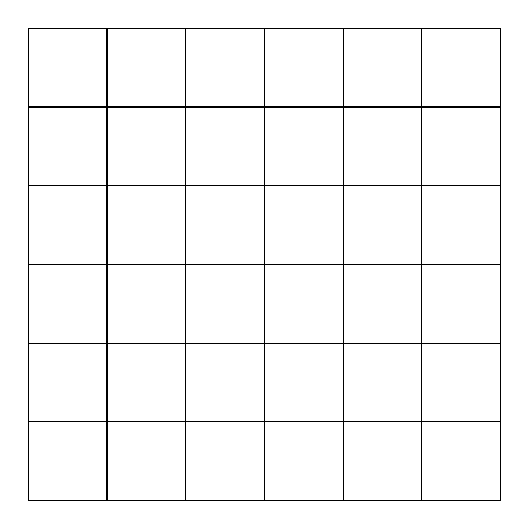
\begin{tikzpicture}
    \draw (0,0) grid (6,6);
    \end{tikzpicture}
    \end{center}
\end{extraPuzzle}






\begin{puzzleSolutions}
FOR STAFF USE ONLY

Main puzzle solution: ALABAMA MOVED EAST

To grade the Extra,
first check that the dominos are numbered legally. Then check
that no further moves are possible. Disqualify any submissions which fail
either check. Otherwise, record the number of dominos used; the smallest
submission wins.
\end{puzzleSolutions}
